\section{Problem 4: Diatomic Linear Chain}

\subsection{Results}

\subsubsection{Numerical and Analytical Dispersion - Reduced Zone Scheme}
%
The numerical and analytical dispersions are shown in Fig. (\ref{reduced_zone_scheme}) in the reduced zone scheme, i.e. all frequencies are placed within the 1\textsuperscript{st} Brillouin zone. The upper branch is the optical branch, and the lower branch is the acoustic branch.
\begin{figure}[h]
    \centering
    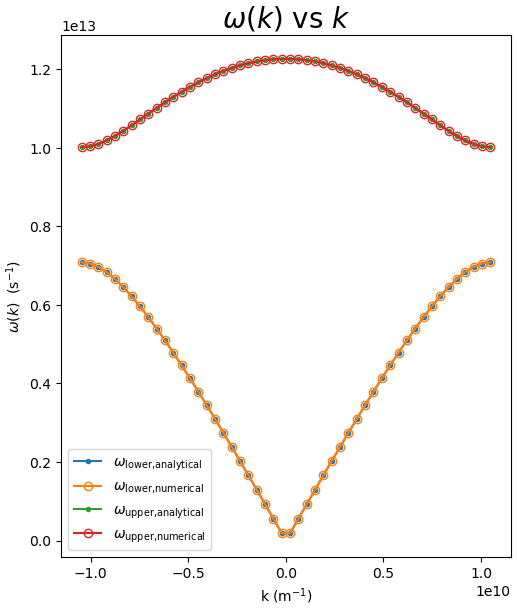
\includegraphics[width=10cm]{reduced_zone_scheme.png}
    \caption{Reduced Zone Scheme for a Diatomic Linear Chain}
    \label{reduced_zone_scheme}
\end{figure}
\begin{table}[h]
\begin{center}
    \footnotesize
    \begin{tabular}{|c|c|c|}
        \hline
        \textbf{System Parameter} & \textbf{Value} & \textbf{Notes} \\ \hline
        Mass 1 & 1.99$\times 10^{-26}$ kg & Mass of One (1) Carbon Atom \\ \hline
        Mass 2 & 2(1.99$\times 10^{-26}$) kg & Mass of Two (2) Carbon Atoms \\ \hline
        Spring Constant & 1 & arbitrary \\ \hline
        Lattice Constant & 3$\times 10^{-10}$ m & arbitrary \\ \hline
        No. of Wavevector Grid Points & 50 & - \\ \hline
    \end{tabular}
\end{center}
\caption{System Parameters for Fig. (\ref{reduced_zone_scheme})}
\label{system_parameters_for_diatomic_linear_chain}
\end{table}


\subsection{Discussion}

Two dispersion values can be found for every wavevector value $k$ in the diatomic linear chain since every unit cell in the diatomic linear chain has two degrees of freedom.